Predstavljene topologije dreves bodo uporabljene za izdelavo podatkovne strukture, ki je ekvivalentna Priponskemu drevesu. Nova podatkovna struktura se imenuje Kompaktno priponsko drevo (angl. \textit{Compressed Suffix Trees} oziroma CST).

Sledeča definicija Sadakane \cite{Sadakane2007} definira abstraktno podatkovno strukturo priponsko drevo in poda vse operacije, ki so potrebne za pravilno delovanje priponskega drevesa.

\begin{defi}\label{def:AST}
    Abstraktna podatkovna struktura Priponsko drevo nad besedilo $T$ podpira sledeče operacije:
    \begin{enumerate}
        \item $koren()$: vrne koren priponskega drevesa,
        \item $jeList(v)$: vrne »Da«, če je vozlišče list, sicer vrne »Ne«,
        \item $otrok(v,z)$: vrne otroka $w$, katerega povezava se začne z znakom $z$. Če otrok ne obstaja vrne 0,
        \item $prviOtrok(v)$: vrne vozlišče $w$, ki je prvi otrok vozlišča $v$,
        \item $nbrat(v)$: vrne vozlišče $w$, ki je naslednji brat od vozlišča $v$,
        \item $pbrat(v)$: vrne vozlišče $w$, ki je predhodni brat od vozlišča $v$,
        \item $star\textit{š}(v)$: vrne vozlišče $w$, ki je starš od vozlišča $v$,
        \item $povezava(v,i)$: vrne $i$-to črko na povezavi do vozlišča $v$,
        \item $globinaNiza(v)$ vrne število znakov na poti iz korena do vozlišča $v$,
        \item $lca(v,w)$: vrne najnižjega skupnega prednika od $v$ in $w$,
        \item $sl(v)$: vrne vozlišče $w$, na katerega kaže priponska povezava iz vozlišča $v$.
    \end{enumerate}
\end{defi}

Kasai idr. \cite{Kasai2001} so predstavili način simulacije priponskega drevesa s pomočjo priponskega polja (angl. \textit{Suffix Array} oziroma SA) in polja najdaljših skupnih predpon (angl. \textit{Longest Common Preffix} oziroma LCP). Z uporabo kompaktnih različic teh dveh podatkovnih struktur je možno implementirati kompaktno priponsko drevo. Veliko operacij iz Definicije \ref{def:AST} so operacije nad drevesi, zato je potrebno dodati še kompaktno predstavitev topologije drevesa, saj le ta pospeši operacije nad drevesi. Torej sledi definicija za podatkovno strukturo kompaktno priponsko drevo.

\begin{defi}
    Kompaktno priponsko drevo nad besedilom $T$ je sestavljeno iz sledečih podatkovnih struktur:
    \begin{enumerate}
        \item topologija drevesa $\tau$,
        \item kompaktno priponsko polje $SA$, %stisnjeno priponsko polje %
        \item kompaktna predstavitev polja najdaljših skupnih predpon $LCP$.
    \end{enumerate}
\end{defi}

V nadaljevanju poglavja bo predstavljena Sadakanejeva \cite{Sadakane2007} implementacija kompaktnega priponskega drevesa. V Poglavju \ref{sec:kompaktna_drevesa} je bilo predstavljenih več različnih predstavitev topologije dreves, implementacija kompaktnega priponskega drevesa pa uporablja predstavitev z zaporedjem uravnoteženih oklepajev.

Topologija drevesa mora podpirati operacije $rang_p$, $izbira_p$, $zapri$, $odpri$ in $oklepa$, ki se izvajajo v konstantnem času za $p\in\{0,1\} ^*$. Pri tem so potrebne dve dodatni podatkovni strukturi za operacijo $rang$ ( $rang_0$, $rang_{01}$) in tri za operacijo $izbira$ ($izbira_0$, $izbira_1$ in $izbira_{01}$). Ostale operacije pa uporabljajo podatkovno strukturo za višek predstavljeno v \cite{Munro1997}, ki je implementirana na podoben način kot dodatna podatkovna struktura za $rang$, namesto $rmM$-drevesa. To pomeni, da za operacijo $otrok(v,i)$ je potrebno $O(|\Sigma|)$ časa. Zato tudi operacija $lca(v,w)$ potrebuje dodatno podatkovno strukturo, ki ji omogoča konstanten čas izvajanja. Ta podatkovna struktura potrebuje $o(n)$ dodatnih bitov. Dodatna podatkovna struktura $L$ za operacijo $lca(v,w)$ deluje na podoben način kot podatkovna struktura za $rang$, pri čemer $L[i]$ je višek na vzorčnem mestu $i$. Za hitrejše delovanje operacije se zgradi še dvodimenzionalno tabelo $M[i,k]$, ki  shrani položaj najmanjšega viška na intervalu $L[i..i+2^k-1]$. Vrednost $k$ je manjša od velikosti vedra. Torej operacija $lca(v,w)$ se izračuna kot $\min\{M[v',k],M[w'-2^k+1,k]\}$, pri čemer je $k=\lfloor \log{(w'-v')\rfloor}$, $v'$ predstavlja vedro v $L$, ki vsebuje $v$, ter $w'$ je vedro v $L$, ki vsebuje $w$. 

V primeru, da so potrebne dodatne operacije, ki temeljijo na $rMq$ operaciji in $|\Sigma|>\log{n}$, se lahko doda še $rmM$-drevo, ki omogoča izvedbo operaciji v $O(\log{n})$ ter pospeši izvajanje oziroma omogoča implementacijo tudi drugih operacij.

\begin{lema}\label{lema:BP}
 Podatkovna struktura za predstavitev topologije priponskega drevesa $\tau$ nad besedilom $T$ dolžine $n$ potrebuje $4n+o(n)$ bitov.
\end{lema}

\begin{proof}
Priponsko drevo nad besedilom $T$ ima $2n-1$ vozlišč: od tega je $n-1$ notranjih vozlišč in $n$ listov. Zato je potrebnih $4n-2$ bitov za zapis topologije drevesa $\tau$ s sekvenco uravnoteženih oklepajev. Torej celotna podatkovna struktura topologije drevesa potrebuje $4n+o(n)$ bitov, saj vsaka dodatna podatkovna struktura potrebuje še dodatnih $o(n)$ bitov.
\end{proof}

Naslednja podatkovna struktura, ki je potrebna za pravilno delovanje kompaktnega priponskega drevesa, je kompaktno priponsko polje (angl. \textit{Compressed Suffix Array} oziroma CSA). Priponsko polje (angl. \textit{Suffix Array} oziroma SA) je podatkovna struktura, v kateri so shranjene vse pripone besedila $T$ v leksikografskem vrstnem redu. Priponska polja so implementirana kot polje indeksov začetkov pripon (cela števila), torej potrebujejo $O(n\log{n})$ bitov (v praksi $O(nw)$ bitov, saj implementacije uporabljajo prevzeto dolžino celega števila). Kompaktna priponska polja znižajo prostorsko zahtevnost na $O(n\log{|\Sigma|})$ bitov \cite{Grossi2000} ali celo na $nH_h +o(n)$ bitov \cite{Grossi2003}, pri čemer je red $h\le\alpha\log_{|\Sigma|}{n};0<\alpha<1$ in $H_h$ je entropija $h$-tega reda, ki se v praksi uporablja kot merilo prostorske zahtevnosti pri kodiranju besedil \cite{Navarro2016}.

Obstajata dve različici kompaktnih priponskih polj: prva implementacija temelji na funkciji $\Psi$, druga implementacija imenovan $FM$-indeks pa uporablja $LF$ funkciji, ki je inverzna funkcija od $\Psi$ \cite{Navarro2016, Sadakane2007}.

Implementacije kompaktnega priponskega polja, ki so lahko uporabljajo pri implementaciji kompaktnih priponskih dreves, morajo podpirati sledeče operacije.

\begin{defi}\label{def:csa}
     Kompaktno priponsko polje nad besedilom $T$, ki je uporabljeno za predstavitev kompaktnega priponskega drevesa, podpira sledeče operacije:
    \begin{enumerate}
        \item $pripona(i)$ vrne $SA[i]$ v času $t_{SA}$,
        \item $inverz(i)$ vrne $j=SA^{-1}[i]$, pri čemer je $SA[j]=i$, v času $t_{SA}$,
        \item $\Psi(i)$ vrne $SA^{-1}[SA[i]+1]$ v času $t_\Psi$,
        \item $besedilo(i,d)$ vrne $T[SA[i]:SA[i]+d-1]$ v času $O(dt_\Psi)$.
    \end{enumerate}    
\end{defi}

Funkcija $\Psi$ je uporabna v kompaktnih priponskih drevesih za izgradnjo priponskih povezav v konstantnem času oziroma v času $t_\Psi$, čeprav ni potrebna za pravilno delovanje kompaktnega priponskega polja. Iz definicije funkcije $\Psi$ je razvidno, da jo lahko simuliramo z uporabo operacij $inverz(i)$ in $pripona(i)$. Iz definicije \ref{def:csa} sledi, da mora kompaktno priponsko polje podpirati funkcijo $\Psi$, zato implementacije z $FM$-indeksom ne pridejo v poštev. 

Vse štiri operacije so lahko implementirane z uporabo $\Psi$ funkcije ter z vzorčenjem priponskega polja $SA$ in inverznega priponskega polja $SA^{-1}$. Na ta način ni potrebno hraniti besedila $T$ in celotnega priponskega polja $SA$.

Funkcija $\Psi$ je predstavljena z istoimenskim poljem, katerega $i$-ta celica je $\Psi[i]=\Psi(i)=SA^{-1}[SA[i]+1]$. Ideja kompaktnega zapisa polja $\Psi$ temelji na dejstvu, da za $j=SA[i]$ in $j'=SA[i+i]$ ter $T[j]=T[j']$ sledi $T[j+1,n]<T[j'+1,n]$ (leksikografsko), torej tudi $\Psi(i)<\Psi(i+1)$. 

Dejstvo se lahko zapiše: kot bitno polje $D$, pri čemer $D[i]=1$, ko je $i=1$ ali $T[SA[i]]\ne T[SA[i+1]]$, ter polje znakov $S$ urejenih v leksikografskem vrstnem redu, tako da $T[SA[i]]=S[rang(D,i)]$.

Polje $\Psi$ se lahko razdeli na $|\Sigma|$ delov in uvede polje $C$, za katerega velja $C[c]=i$, tako da $T[SA[i+1]]=c$ in $T[SA[i]]\ne c$, za vsak $c\in\Sigma$. Polje $C$ potrebuje $O(|\Sigma|\log{n})$ bitov. Tako se lahko razdeli $\Psi$ na $\Psi_c;\:c\in\Sigma$, kjer je $\Psi[i]=\Psi_c[i']$,  za $i'=i-C[S[rang_1(D,i)]]$. Vsako polje $\Psi_c$ se lahko zapiše kot bitno polje $B_c$ dolžine $n$, pri čemer $B_c[\Psi_c[i]]=1$ za $1 \le i \le n_c$, kjer je $n_c$ število ponovitev znaka $c$ v besedilu $T$. Torej velja $\Psi_c[i']=izbira_1(B_c,i')$ ali $\Psi[i]=izbira_1(B_c,i-C[c])$, kjer $c=rang_1(D,i)$. Bitna polja $B_c$ so zelo redka (število enic je bistveno manjše kot število ničel), torej se jih lahko stisne iz $|\Sigma|n+o(n)$ bitov na $n_c\log\frac{n}{n_c}+O(n_c)$ bitov, kar pomeni, da funkcija $\Psi$ potrebuje $nH_0(T)+O(n+|\Sigma|w)$ bitov, pri čemer $H_0(T)$ je entropija besedila $T$ \cite{Navarro2016}.

Do sedaj predstavljena podatkovna struktura omogoča zgolj iskanje števila ponovitev vzorca v besedilu, ne pa lokacije pojavov vzorca v besedilu. Za to sta potrebni dodatni podatkovni strukturi, ki nadomestita priponsko polje $SA$ ter inverzno polje $SA^{-1}$. Priponsko polje $SA$ se vzorči $l=\Theta(\log{n})$-krat. Pri tem se uporabi dodatno bitno polje $B$, kjer $B[i]=1$ natanko tedaj, ko $i=1$ ali $SA[i]\mod{l} =0$. Polje vzorcev $SA_S$ vsebuje vrednosti $SA_S[rang_1(B,i)]=SA[i]$, ko je $B[i]=1$. Ostale vrednosti $SA[i]$ se izračuna kot $SA[i]=SA_S[rang_1(B,i_k)]-k$, pri čemer je $i_k$ $k$-kratna aplikacija funkcije $\Psi$ oziroma $i_k=\Psi^k[i]$ (na primer $i_2=\Psi^2[i]=\Psi[\Psi[i]]$) \cite{Navarro2016}.

Podobno se vzorči tudi polje inverzov pripon $SA^{-1}$ le da se ta vzorči na enakomernih intervalih dolžine $l$. Polje vzorcev $SA^{-1}_S[1:\lfloor n/l\rfloor]$ se uporabi za izračun vrednoti $SA^-1[i]$. Najprej izračuna $i'=\lfloor i/l\rfloor l$, nato se $i-i'$-krat aplicira funkcija $\Psi$ nad vrednostjo $j'=SA^{-1}_S[i'/l]$ oziroma $\Psi^{i-i'}[SA^{-1}_S[i'/l]]$ \cite{Navarro2016}.

Tako predstavljeno kompaktno priponsko polje potrebuje $nH_0(T)+O(n+|\Sigma|w)$ bitov za implementacijo. Potrebni čas za izračun funkcije $\Psi$ je $t_\Psi=O(1)$ ter potrebni čas za iskanje po priponskem polju in inverznem priponskem polju je $t_{SA}=t_\Psi \log{n} = O( \log{n})$.

Zadnja podatkovna struktura, ki sestavlja kompaktno priponsko drevo, je polje najdaljših skupnih predpon (angl. \textit{Longest Common Prefixs} oziroma $LCP$). V polju so shranjene dolžine najdaljše predpone dveh zaporednih pripon. Polje $LCP[2,n]$ dolžine $n-1$ je sestavljeno iz celic z vrednostjo
$$
    LCP[i]=lcp(SA[i-1],SA[i]);\:2\le i\le n,
$$
pri čemer je funkcija $lcp(X,Y)=\max\{i;X[1,i]=Y[1,i]\}$. Polje $LCP$ je lažje shraniti kot permutacijo $PLCP$, pri čemer $PLCP[i]=LCP[SA^{-1}[i]]$ ali $LCP[i]=PLCP[SA[i]]$  \cite{Navarro2016}.


Permutacijo $PLCP[1,n-1]$ je lažje shraniti, saj je zaporedje $PLCP[i]+2i$ za vsak $i$ med $1$ in $n-1$ strogo naraščajoče. Saj je $PLCP[i+1]\ge PLCP[i]-1$. To enostavno dokažemo, saj obstajata $T[j,n]$ in $T[i,n]$, $T[i,n]<T[j,n]$, ki imata najdaljšo skupno predpono dolžine $PLCP[i]>0$. Potem ima $T[i+1,n]$ najdaljšo skupno predpono s $T[j+1,n]$ dolžine $PLCP[i]-1$ in vsi nizi, ki so leksikografsko med $T[i+1,n]$ in $T[j+1,n]$, imajo najdaljšo skupno predpono s $T[i+1,n]$ vsaj dolžino $PLCP[i]-1$. Torej je $PLCP[i+1]\ge PLCP[i]-1$ in še vedno velja $PLCP[i]+2i<PLCP[i+1]+2(i+1)\le PLCP[i]+2i+1$. Ker je $PLCP[n-1]+2(n-1)< 2n$, saj $T[n-1,n]$ ima lahko dolžino najdaljše skupne predpone 1, s poljubno pripono, se lahko permutacijo $PLCP$ in posledično $LPC$ polje zapiše kot bitno polje $H[1,2n-1]$. Celica $H[j]=1$ za $j=PLCP[i]+2i$, kjer je $i$ med $1$ in $n-1$. Pri tem bitno polje $H$ potrebuje dodatno podatkovno strukturo za $izbiro_1$ \cite{Navarro2016}.

Vrednost $LCP[i]$ se lahko pridobi v $O(\log{n})$ času. Vrednost je izračunana z uporabo formule $LCP[i]=izbira_1(H,SA[i])-2SA[i]$. Operacija potrebuje $O(\log{n})$ časa, saj je potrebno izračunati vrednost $SA[i]$, ki se jo izračuna v $O(\log{n})$ času, ostale operacije pa potrebujejo konstanten čas. 

Prostorska zahtevnost polja $LCP$ je predstavljena s sledečo lemo:

\begin{lema}\label{lema:LCP}
 Podatkovna struktura $LCP$ potrebuje $2n+o(n)$ bitov za pravilno delovanje.
\end{lema}

\begin{proof}
    Podatkovna struktura $LCP$ je shranjena kot bitno polje $H[1,2n-1]$. Bitno polje $H$ potrebuje dodatnih $o(n)$ bitov za dodatno podatkovno strukturo, ki omogoča izvajanje operacije $izbira_1$ v konstantnem času. Ker je bitno polje $H$ dolžine $2n-1$ in potrebuje dodatnih $o(n)$ bitov, potem celotna podatkovna struktura za shraniti polje $LCP$ potrebuje $2n+o(n)$ bitov.
\end{proof}

Sedaj, ko so bile predstavljene vse podatkovne strukture, ki sestavljajo kompaktno priponsko drevo, je možno izračunati velikost celotnega kompaktnega priponskega drevesa. Ker obstaja več implementacij kompaktnega priponskega polja, ki se lahko uporabijo v kompaktnem priponskem drevesu, bo velikost priponskega drevesa vsebovala člen $|CSA|$, ki predstavlja velikost kompaktnega priponskega polja. Velikost kompaktnega priponskega drevesa je predstavljena v sledečem izreku:

\begin{izr}
    Podatkovna struktura kompaktno priponsko drevo nad besedilom $T$ dolžine $n$ potrebuje $|CSA|+6n+o(n)$ bitov, pri čemer $|CSA|$ predstavlja velikost kompaktnega priponskega polja.
\end{izr}
\begin{proof}
    Ker obstajajo različne implementacije kompaktnega priponskega polja, je potrebnih $|CSA|$ bitov za shraniti kompaktno priponsko polje $SA$. Iz Leme \ref{lema:BP} sledi, da je potrebnih $4n+o(n)$ bitov za shraniti topologijo drevesa $\tau$. Iz Leme \ref{lema:LCP} pa sledi, da je potrebnih $2n+o(n)$ bitov za shraniti polje $LCP$.

    Torej velikost kompaktnega priponskega drevesa $CST$ je $|CSA|+6n+o(n)$.
\end{proof}

Obstaja več različnih implementacij kompaktnega priponskega polja, zato Sadakane \cite{Sadakane2007} predlaga dve implementaciji. Prva predlagana implementacija je prostorsko učinkovita in uporablja kompaktno priponsko polje, ki so ga predlagali Grossi idr. \cite{Grossi2003}. 

\begin{posl}\label{pos:CSAnh}
Kompaktno priponsko drevo implementirano s pomočjo kompaktnega priponskega polja, ki potrebuje $|CSA|=nH_h+O(n\log\log{n} / \log_{| \Sigma|}{n})$ bitov, potrebuje $|CST|= nH_h+6n+O(n\log\log{n} / \log_{| \Sigma|}{n})$ bitov.    
\end{posl}

Druga predlagana implementacija pa je časovno učinkovita in uporablja kompaktno priponsko polje, ki ga sta ga predlagala Grossi in Vitter \cite{Grossi2000}. 
\begin{posl}\label{pos:CSAlog}
Kompaktno priponsko drevo implementirano s pomočjo kompaktnega priponskega polja, ki potrebuje $O(\frac{1}{\epsilon}n\log{| \Sigma|})$ bitov, potrebuje $|CST|=O(\frac{1}{\epsilon}n\log{| \Sigma|})$ bitov. Pri tem je $\epsilon$ poljubna konstanta, ki ima vrednost $0<\epsilon<1$.
\end{posl}

\begin{figure}[tb]
    \begin{center}
        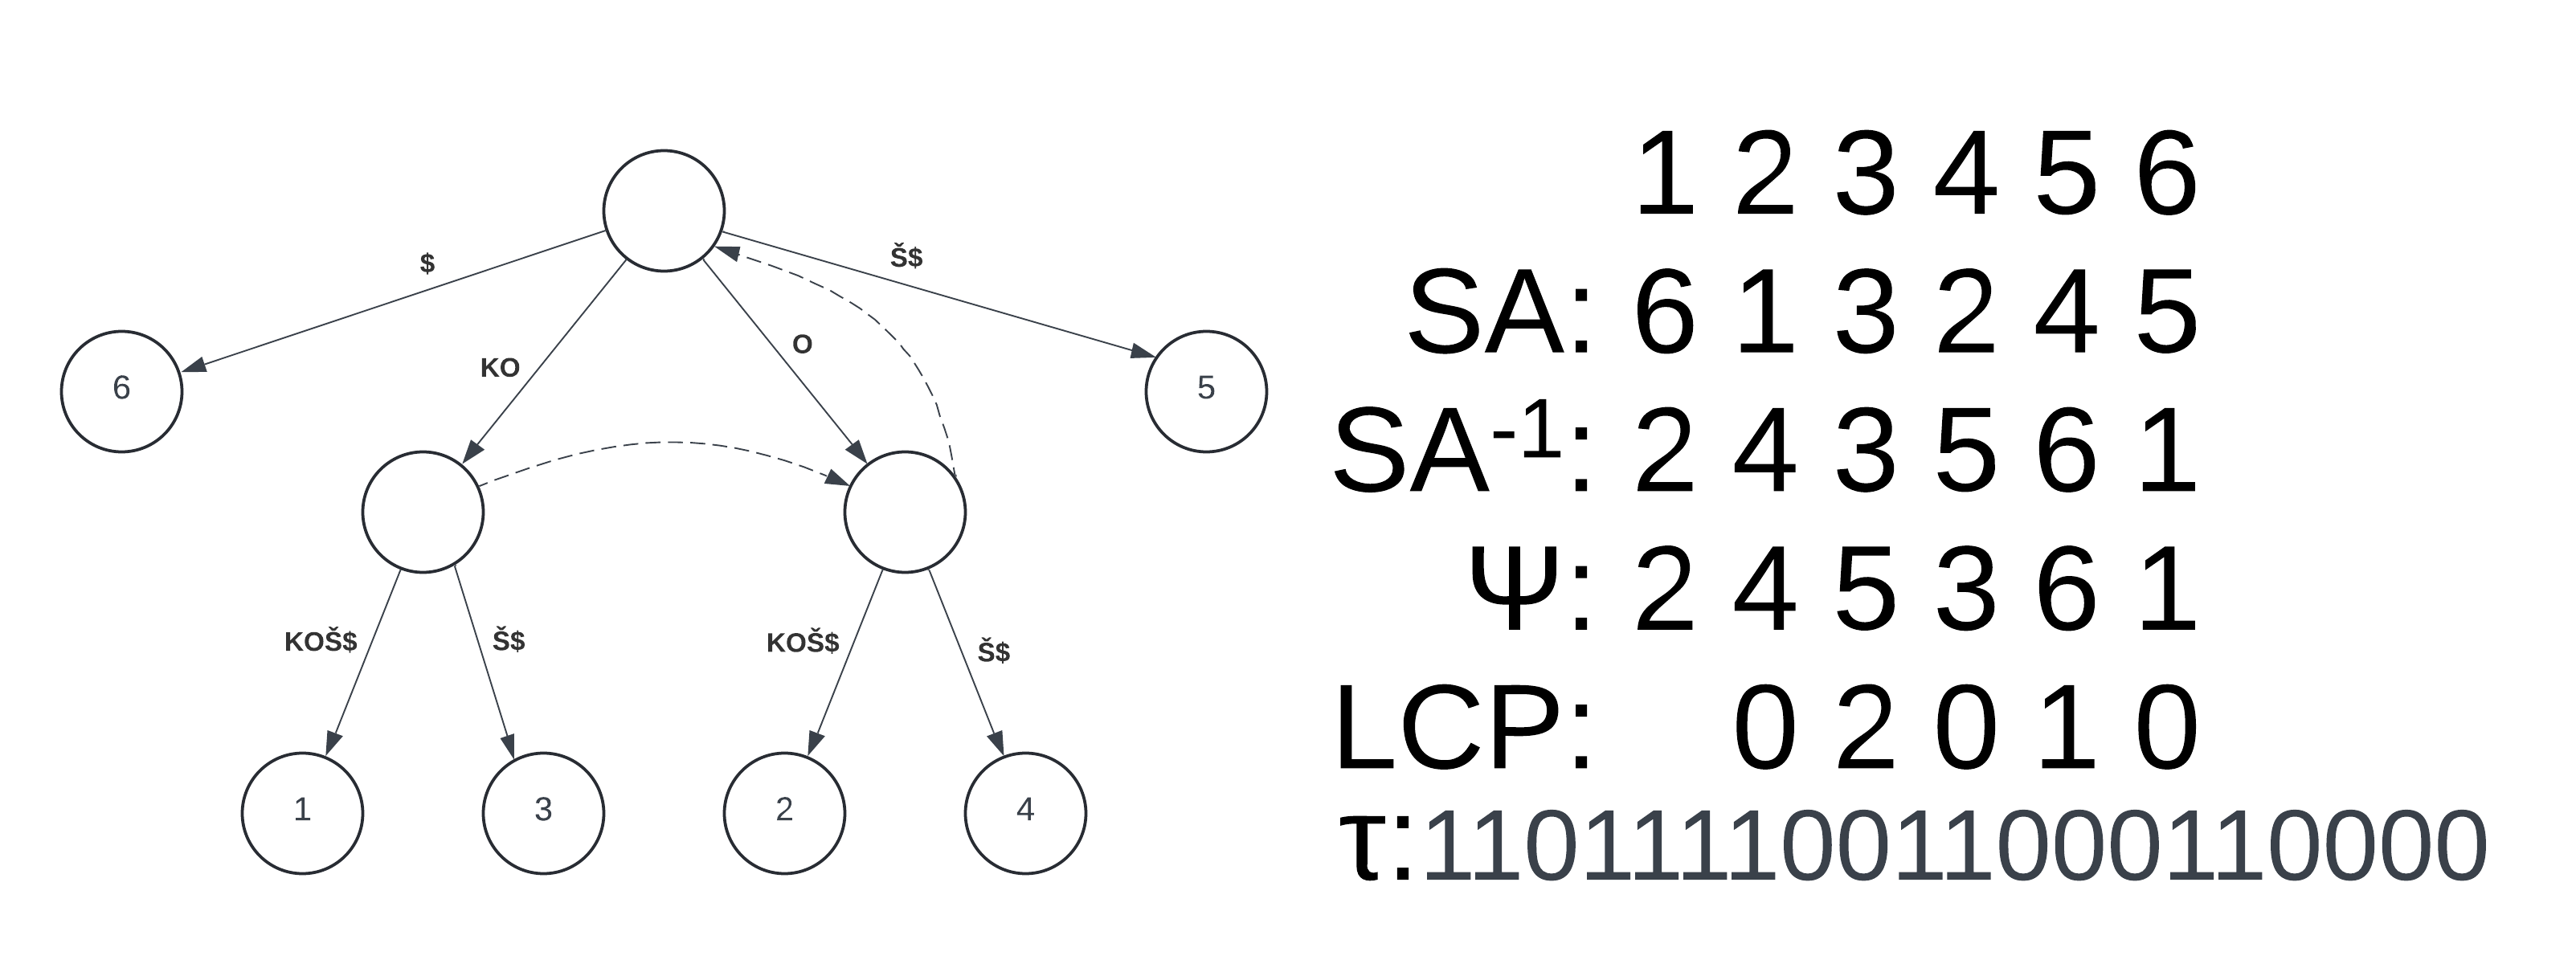
\includegraphics[width=1.03\textwidth]{Slike/KokosCST.png}
        \captionof{figure}[Primer priponskega drevesa (levo) in kompaktnega priponskega drevesa (desno) za besedo »KOKOŠ$\$$«. ]{Primer priponskega drevesa (levo) in kompaktnega priponskega drevesa (desno) za besedo »KOKOŠ$\$$«.} 
        \label{fig:CST}
    \end{center}
\end{figure}

Primer kompaktnega priponskega drevesa je prikazan na Sliki \ref{fig:CST}. Zaradi lažje berljivosti so vse komponente kompaktnega priponskega drevesa (na desni strani slike) prikazane v ne kompaktni obliki. Priponsko polje je prikazano v treh vrsticah (vrstica, ki se začne s $SA$, vrstica, ki se začne s $SA^{-1}$, in vrstica ki se začne s $\Psi$).

Prostorsko zahtevnost kompaktnega priponskega drevesa je možno še dodatno znižati na $|CSA|+o(n)$. Russo idr. \cite{Russo2008} so predstavili način kako doseči to prostorsko zahtevnost. To so dosegli, tako da so vzorčili $O(n/\delta)$ vozlišč, pri čemer $\delta=\omega(\log_{|\Sigma|}{n})$ in predstavlja faktor vzorčenja. Vzorčeno drevo potrebuje $o(n)=O(n/\log_{|\Sigma|}{n})$ bitov. Poleg vzorčenja topologije drevesa, so se znebili tudi $LCP$ polja. To jim je omogočalo znižanje prostorske zahtevnosti iz $|CSA|+6n+o(n)$ bitov na $|CSA|+o(n)$ bitov. Na ta račun pa se je dvignila časovna zahtevnost nekaterih operacij, ki so bile prej izvršene v konstantnem času.


\subsection{Izgradnja}\label{sec:CSTizgradnja}
\import{.}{KompaktnaPredstavitev/Izgradnja}



